\documentclass[tikz,border=12pt]{standalone}
\usepackage{amsmath,amssymb}
\usetikzlibrary{calc,arrows.meta}

\begin{document}
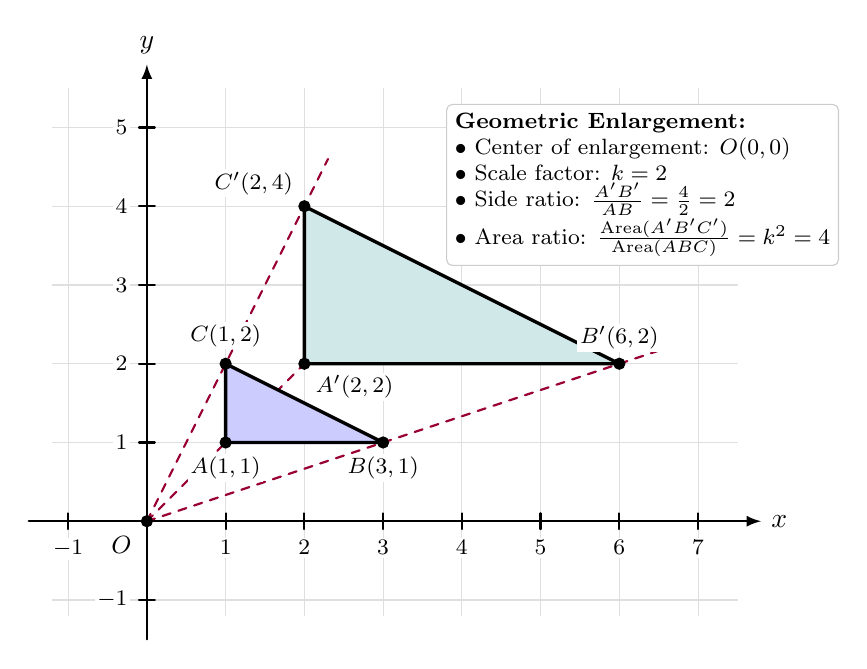
\begin{tikzpicture}[>=latex, line cap=round, line join=round]
  % Grid
  \draw[step=1cm, gray!25, thin] (-1.2, -1.2) grid (7.5, 5.5);

  % Axes
  \draw[thick, ->] (-1.5, 0) -- (7.8, 0) node[right, font=\normalsize] {$x$};
  \draw[thick, ->] (0, -1.5) -- (0, 5.8) node[above, font=\normalsize] {$y$};

  % Origin
  \node[below left=2pt, font=\small] at (0, 0) {$O$};

  % Integer ticks on x-axis
  \foreach \x in {-1,1,2,3,4,5,6,7} {
    \draw[thick] (\x, 0.1) -- (\x, -0.1);
    \node[below=3pt, font=\footnotesize, fill=white, inner sep=1pt] at (\x, -0.1) {$\x$};
  }
  % Integer ticks on y-axis
  \foreach \y in {-1,1,2,3,4,5} {
    \draw[thick] (0.1, \y) -- (-0.1, \y);
    \node[left=3pt, font=\footnotesize, fill=white, inner sep=1pt] at (-0.1, \y) {$\y$};
  }

  % Coordinates
  % Center of Enlargement
  \coordinate (O) at (0, 0);

  % Pre-image triangle ABC
  \coordinate (A) at (1, 1);
  \coordinate (B) at (3, 1);
  \coordinate (C) at (1, 2);

  % Image triangle A'B'C' (scale factor k = 2)
  \coordinate (A1) at (2, 2);
  \coordinate (B1) at (6, 2);
  \coordinate (C1) at (2, 4);

  % Projection rays from center O through object vertices to image vertices
  \draw[thick, dashed, purple!80!black] (O) -- (2.5, 2.5);
  \draw[thick, dashed, purple!80!black] (O) -- (6.6, 2.2);
  \draw[thick, dashed, purple!80!black] (O) -- (2.3, 4.6);

  % Image triangle A'B'C' (drawn first so object sits crisply)
  \draw[very thick, fill=teal!18] (A1) -- (B1) -- (C1) -- cycle;
  \filldraw[black] (A1) circle (2pt) node[below right=3pt, font=\footnotesize\bfseries, fill=white, inner sep=1pt] {$A'(2,2)$};
  \filldraw[black] (B1) circle (2pt) node[above=4pt, font=\footnotesize\bfseries, fill=white, inner sep=1pt] {$B'(6,2)$};
  \filldraw[black] (C1) circle (2pt) node[above left=3pt, font=\footnotesize\bfseries, fill=white, inner sep=1pt] {$C'(2,4)$};

  % Object triangle ABC
  \draw[very thick, fill=blue!20] (A) -- (B) -- (C) -- cycle;
  \filldraw[black] (A) circle (2pt) node[below=4pt, font=\footnotesize\bfseries, fill=white, inner sep=1pt] {$A(1,1)$};
  \filldraw[black] (B) circle (2pt) node[below=4pt, font=\footnotesize\bfseries, fill=white, inner sep=1pt] {$B(3,1)$};
  \filldraw[black] (C) circle (2pt) node[above=5pt, font=\footnotesize\bfseries, fill=white, inner sep=1pt] {$C(1,2)$};

  % Center point marker
  \filldraw[black] (O) circle (2pt);

  % Annotations block
  \node[align=left, font=\footnotesize, fill=white, inner sep=3pt, draw=gray!40, rounded corners=2pt, anchor=north west] at (3.8, 5.3) {
    \textbf{Geometric Enlargement:}\\
    $\bullet$ Center of enlargement: $O(0,0)$\\
    $\bullet$ Scale factor: $k = 2$\\
    $\bullet$ Side ratio: $\frac{A'B'}{AB} = \frac{4}{2} = 2$\\
    $\bullet$ Area ratio: $\frac{\text{Area}(A'B'C')}{\text{Area}(ABC)} = k^2 = 4$
  };

\end{tikzpicture}
\end{document}
